\documentclass[12pt,a4paper]{article}
\usepackage{amsmath}
\usepackage{mathtext}
\usepackage{icomma}
\usepackage[unicode, pdftex]{hyperref}
\usepackage{amsfonts}
\usepackage{amssymb}
\usepackage[utf8]{inputenc}
\usepackage[T1,T2A]{fontenc}
\usepackage[english, russian]{babel}
\usepackage{graphicx}
\usepackage[left=2cm,right=2cm,top=2cm,bottom=2cm]{geometry}
\usepackage{calc}
\usepackage{wrapfig}
\usepackage{setspace}
\usepackage{indentfirst}
\usepackage{subfigure}
\usepackage[table,xcdraw]{xcolor}

\author{Московский физико-технический интститут\\Исламов Сардор, группа Б02-111}
% \date{6 июня 2022 г.}
\begin{document}	

\begin{center}

    Московский физико-технический интститут

    Физтех-школа физики и исследований им. Ландау

    Исламов Сардор, группа Б02-111
    \vskip 0.5cm   
    \Large{Ислледование явления диссипации атмосфер планет}
\end{center}

\subparagraph*{Аннотация.}
В данной работе исследовано такое явление, как диссипация атмосфер планет. 
Также оценен вклад различных механизмов диссипации в скорость рассеяния атмосферы. 
Предложен новый метод оценки скорости диссипации легких газов и на его основе спрогнозирована продолжительность жизни атмосферы Земли -- 200 лет.

Для исследования были использованы распределения Максвелла, Больцмана и классическая формула Джинса для потока ускользания частиц в космическое пространство. 

Работа состоит из двух разделов: теоретическое введение и построение модели. 
В первом представлены общие понятия строении атмосферы и теоретическая база, необходимая для проведения расчетов.
Во втором разделе проведены расчеты и сама оценка жизни Земной атмосферы.

\subsection*{Теоретичское введение}
Продолжительность жизни нашей атмосферы всегда будет трепещущим вопросом.
Невозможно провести точные расчеты и построить модели, учитывающие всевозможные факторы, влияющие на Земную атмосферу, но можно провести некоторую оценку. 
Так, например, по результатам исследований, В. И. Мороз, советский и российский астроном, доктор физико-математических наук, профессор МГУ, лауреат Государственной премии СССР, в 1967 году спрогнозировал, что время полной диссипации водорода в атмосфере должно было произойти 5 лет назад, к 2017 году.
Данная отсрочка, возможно, частично связана с пополнением ресурсов атмосферы из недр Земли и некоторых химических реакций, продуктом которых является водород.

В работе проведена оценка именно потерь атмосферы без учета вышеупомянутой компенсации, т. к. эти процессы носят скорее химический и вероятностный характер, не относящийся к разделу термодинамики.
Результаты этого исследования вместе с использованием существующих моделей можно использовать в дальнейших исследованиях для оценки вклада выделения из недр Земли газов, диссоциации веществ и прочих аспектов, обновляющих ресурсы.
В данном разделе представлена информация о строении атмосферы Земли, ее слоях и их особенностях, определения диссипации атмосфер планет и различных ее механизмов.

\subparagraph*{Строение атмосферы.}
Атмосфера -- это газовая оболочка планеты, защищающая ее поверхность от космических угроз: метеоритов, радиации, ультрафиолетового излучения и т. д.
По данным на 2020 г. масса атмосферы Земли составляет $\sim 5.2 \cdot 10^{18}\ кг$, из которых сухой воздух составляет около 98\%, а высота атмосферы $\sim 1000\ км$ \cite{Careva}. 
Для лучшего понимания дальнейшей теории ниже перечислены слои атмосферы и основная информация по ним из открытых источников \cite{wiki_atm}.

Тропосфера -- нижний слой атмосферы, содержит в себе более 80\% общей массы воздуха в атмосфере и более 90\% массы водяного пара. 
Верхняя граница тропосферы лежит на высоте от 8 до 18 км в зависимости от широты и времени года.

Тропопауза -- переходный слой от тропосферы к стратосфере, в котором прекращается снижение температуры воздуха с возрастанием высоты.

Стратосфера -- слой атмосферы, располагающийся на высоте от 11 до 50 км. 
В нижних слоях характерное изменение температуры отсутствует, далее она повышается от $-56.5$°C до $+0.8$°C.
Температура около нуля по цельсию сохраняется в интервале 40-55 км, который называется стратопаузой.
Также этот слой является переходным от стратосфере к мезосфере.

Мезосфера простирается от 50 до 80-90 км.
Температура с возрастанием высоты понижается со средним градиентом $\sim 3 \cdot 10^{-3} {^oC \over м}$.

Мезопауза -- переходный слой атмосферы от мезосферы к термосфере. 
Локальный минимум температуры около $-90$°C.

Верхний слой атмосферы - термосфера, простирается до уровня 800 км.
Температура растет до высот 200-300 км, где достигает значений порядка 1000 К, после чего остается почти постоянной до больших высот.
\vskip 0.5 cm
До высоты 100 км атмосфера представляет собой гомогенную хорошо перемешанную смесь газов. 
В более высоких слоях распределение газов по высоте зависит от их молекулярных масс, концентрация более тяжёлых газов убывает быстрее по мере удаления от поверхности Земли. 
Вследствие уменьшения плотности газов температура понижается от 0°C в стратосфере до --110°C в мезосфере. 
Однако кинетическая энергия отдельных частиц на высотах 200—250 км соответствует температуре $\sim$ 150°C. 
Выше 200 км наблюдаются значительные флуктуации температуры и плотности газов во времени и пространстве. \cite{wiki_atm}
На Рис. 1 изображена зависимость параметров воздуха от высоты.

\begin{figure}[htp]
    \centering
    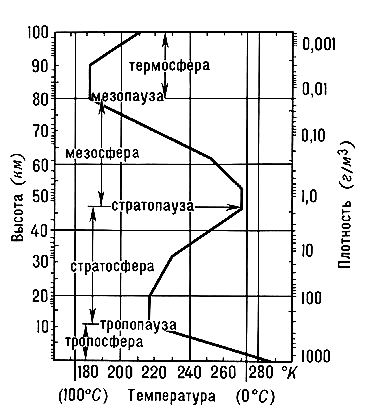
\includegraphics[width=0.6\linewidth]{atmosphere_layers.png}
    \caption{Зависимость давления и температуры воздуха от высоты \cite{pressure}}
\end{figure}

В верхних слоях атмосфера плавно переходит в межпланетное пространство -- экзосферу, при этом ее плотность и концентрация падают.
Высота, сравнимая с величиной длины свободного пробега молекул при данной температуре, то есть с средним расстоянием, преодолеваемым молекулой между двумя последовательнымы ударами, называется экзобазой -- это и есть граница раздела атмосферы и нижней границей экзосферы. 
Длина свободного пробега вычисляется по формуле
\begin{equation}
    \lambda = {1 \over n \sigma},
\end{equation}
где $n$ -- концентрация частиц в рассматриваемой области, $\sigma \sim d^2$ -- эффективное сечение, где $d$ -- диаметр молекулы.
На уровне экзобазы частицы, обладающие достаточной радиальной скоростью -- выше критической скорости ускользания, равной второй космической скорости $v_2 = \sqrt {2G{M_\oplus \over R_\oplus}}$ -- имеют высокую возможность навсегда покинуть атмосферу Земли, не встретив более частиц на своем пути.
Такое явление рассеивания атмосферы и называется ее диссипацией.
Устойчивой считается атмосфера, средняя скорость молекул которой не превышает 0.2 от критической. 
% Если порог средней тепловой скорости составляет 0.25 от критической, то атмосфера рассеивается за 50000 лет, а если 0.33 от критической - в течение всего нескольких недель.
Существуют различные механизмы диссипации, речь о которых и пойдет дальше.

\subparagraph*{Термальный механизм диссипации.}
При тепловой диссипации высокая скорость частиц, покидающих атмосферу, обусловлена локальной температурой.
Согласно работе Шематовича и Ярова (2018) \cite{schem}, если атмосфера вблизи экзобазы находится в гидростатическом равновесии, то распределение скоростей частиц в этой области соответствует распределению Максвелла:
\begin{equation}
    f(v)dv = 4 \pi v^2 \left({m \over 2\pi k T}\right)^{3/2} \exp\left({m v^2 \over 2kT}\right)dv.
\end{equation}
Такой механизм диссипации носит название диссипации Джинса и характерен для более легких частиц. 
В этом случае поток убегания на высоте экзобазы описывается классической формулой Джинса:
\begin{equation}
   F_e(r_e) = {\rho(r_e) v_{н.в.}\over 2 \sqrt \pi}(\beta + 1)e^{-\beta},
\end{equation}
где $\rho(r_e)$ -- плотность на высоте экзобазы, причем $r_e = h_e + R_\oplus$ -- расстояние от высоты экзобазы до центра Земли, $v_{н.в.}$ -- наиболее вероятная скорость из распределения Максвелла, а $\beta$ -- безразмерный параметр убегания, равный квадрату отношения критической скорости убегания на высоте экзобазы к наиболее вероятной скорости:
\begin{equation*}
    \beta = {v_e^2 \over v_{н.в.}^2} = {2GM_\oplus\over r_e}{\mu \over 2RT} = {r_e \over H},\ где\ H = {RT\over \mu g}.
\end{equation*}
Предел потока (3) при $\beta \rightarrow 0$ известен как предел Джинса, характеризующий максимальную скорость теплового убегания:
\begin{equation}
    \lim_{\beta \rightarrow 0} F_e(r_e) = {\rho(r_e)v_{н.в.} \over 2 \sqrt \pi} = \frac 1 4 \rho(r_e) \overline{v},
\end{equation}
где $\overline{v} = \sqrt{8RT\over \pi \mu}$ -- средняя скорость из распределения Максвелла.

Также имеет место экстремальная версия этого механизма -- гидродинамическая диссипация, возникающая, когда легкие частицы, подобно жидкости, увлекают за собой более тяжелые посредством столкновений с ними.

\subparagraph*{Нетермальный механизм диссипации.}
Процесс диссипации называется нетепловым, если высокие скорости убегающих частиц достигаются явлениями, независящими от температуры экзобазы. 
Такие явления часто связаны с фотохимией или взаимодействием заряженных частиц и их поведением в электрическом и магнитном полях. 
Фотохимические потери важны для Марса, но не для Земли, т. к. максимальная кинетическая энергия кислорода, приобретаемая в реакции диссоциативной рекомбинации ниже энергии убегания для планеты более массивной, чем Марс. \cite{Careva}

Также в нетермальной диссипации имеет место влияние солнечного ветра. 
Солнечный ветер может передавать кинетическую энергию молекулам атмосферы, придавая им скорость, позволяющие преодалеть гравитацию планеты.
Но для Земли, благодаря ее сильному магнитному полю, такой механизм вносит не такой сильный вклад в рассеивание атмосферы.
Солнечный ветер, состоящий из ионов, отклоняется магнитосферой, так как заряженные частицы движутся вдоль магнитного поля. 
На Земле магнитосфера отклоняет солнечный ветер с эффективным радиусом порядка 10 радиусов Земли, и эта область отражения называется головной ударной волной.
Таким образом, последние модели показывают, что солнечный ветер отвечает не более чем за 1/3 общей нетермической диссипациии. \cite{wiki_leak} 
На Рис. 2 изображена схема отражения солнечного ветра магнитосферой Земли.

\begin{figure}[h!]
    \centering
    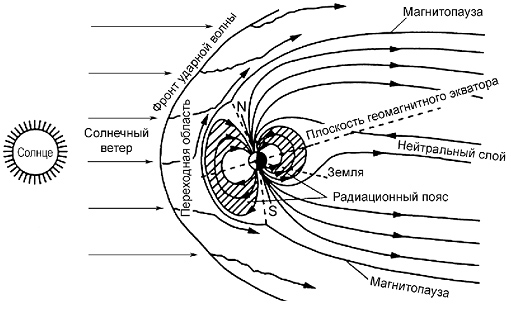
\includegraphics[width=0.65\linewidth]{magnetosphere.jpeg}
    \caption{Магнитосфера Земли \cite{magnet}}
\end{figure}

\newpage

\subsection*{Построение модели}
Как следует из раздела теоретического введения, основной вклад в рассеивание атмосферы планеты вносит именно термальный фактор.
Поэтому проведем оценку скорости ускользания атмосферы на основе термального механизма диссипации.

Из распределения Больцмана становится ясно, что в верхних слоях преобладают частицы с меньшей молекулярной массой, и в первую очередь из нее ускользают гелий, водород и атомарный водород:
\begin{equation}
    n(h) = n_0 \exp{\left(-\mu gh \over RT\right)}
\end{equation}

Оценим длину свободного пробега на высоте $h = 600$ км. 
На данной высоте плотность воздуха порядка $\rho \sim 1 \cdot 10^{-13}\ кг/м^3$ и температура $T \approx 1000$ К. 
Для оценки длины свободного пробега $\lambda$ выразим концентрацию $n$ как функцию от плотности $\rho$, чтобы использовать табличными значения плотности из открытых источников \cite{wiki_standart}:
\begin{equation*}
    n = {N \over V} = {N\rho \over m} = {\rho N \over \mu \nu} = {\rho N \over \mu N/N_A} = {\rho \over \mu}N_A
\end{equation*}

Тогда, взяв молярную массу воздуха $\mu \approx 10\ г/моль$ \cite{mu} и диаметр молекулы водорода $d \approx 0.25$ нм \cite{dh}, из (1) получаем результат, который примерно совпадает с табличными значениями: 
\begin{equation*}
    \lambda = {1 \over n \sigma}\sim {\mu \over \rho N_A \sqrt 2 \pi d^2} \sim 6 \cdot 10^5\ м.
\end{equation*}

Получаем, что длина свободного пробега на уровне $600$ км соизмерима с высотой, для которой проводилcя расчет, то есть это и есть примерный уровень экзобазы.

Теперь расчитаем наиболее вероятную скорость для различных молекул на уровне экзобазы -- при температуре около 1000 К.
Из (2), заменив постоянный коэффициент на $C = 4\pi \left({m\over 2\pi kT}\right)^{3/2}$, получаем, что $f(v) = C v^2 \exp{\left({mv^2 \over 2kT}\right)}$.

В точке максимума, из условия экстремума, ${\partial f(v) \over \partial v} = 0$, тогда, подставляя (2), получим:
\begin{equation*}
    {\partial f(v) \over \partial v} = C \exp{\left({mv^2 \over 2kT}\right)} \left(2v - {mv\over kT}v^2\right) = 0
\end{equation*}
Решив уравнение, получим:
\begin{equation}
    v_{н.в.} = \sqrt{2kT\over m} = \sqrt{2RT\over \mu}.
\end{equation}

В связи с отсутсвием точных данных о процентном содержании водорода на таких высотах сделаем оценку из распределения Больцмана (5).
У поверхности содержание водорода в атмосфере по массе составляет примерно $8 \cdot 10^{-5}\%$.
В таком случае на высоте $h$ процентное соотношение по массе можно расчитать по формуле:
\begin{equation*}
    {m_{H_2} \over m} = {m_{{H_2}_0}\over m_0} \exp\left({\mu-\mu_{H_2} \over RT}gh\right).
\end{equation*}
Проведя расчеты для высоты 100 км, до которой изменения температуры воздуха не столь сущетсвенны, и приняв эту самую температуру за 250 К, получаем число 0.27.
Далее температура довольно быстро достигает значений в 1000 К и остается постоянной, поэтому для высоты порядка 600 км получаем итоговое число $2.2 \cdot 10^{6}$, то есть содержание водорода превосходит содержание кислорода и азота, из которых в основном состоят нижние слои атмосферы, в $2.2\cdot 10^{6}$ раз.
Аналогично для гелия получаем результат $2.5 \cdot 10^{5}$.
В таком случае можем считать, что в атмосфере на такой высоте отсутствуют тяжелые газы, а плотность водорода и гелия в атмосфере составляют соответственно 90\% и 10\% от общей плотности.

Расчитаем утечку водорода и гелия по формуле (3) и занесем данные в Таблицу 1, учитывая, что вторая космическая скорость для Земли $v_2\approx 11.2$ км/с.

\begin{table}[h!]
    \centering
    \begin{tabular}{|c|c|c|c|c|c|c|}
        \hline
        газ & $\mu$, г/моль & $v_{н.в.}$, км/с & $v_{н.в.} / v_2$ & $\sqrt {h_e/H}$ & $F_e,\ 10^{-11}кг / (м^2\cdot c)$\\
        \hline
        $H_2$ & 2 & 2.883 & 0.257 & 0.244 & 14.1\\
        \hline 
        $He$ & 4 & 2.038 & 0.182 & 0.173 & 0.9 \\
        \hline 
        $N_2$ & 28 & 0.770 & 0.069 & 0.065 & --\\
        \hline 
        $O_2$ & 32 & 0.721 & 0.064 & 0.061 & --\\
        \hline 
    \end{tabular}
    \caption{Ускользание различных газов}
\end{table}

Также по полученным значениям проведем оценку времени полной диссипации водорода и гелия из атмосферы.
С площади поверхности атмосферы на уровне экзобазы $S = 4\pi r_e^2 \approx 4.5 \cdot 10^{12}\ м^2$ ежесекундно в космос утекает масса $\mu_- = F_e S$.
Зная массу $m$ всего газа в атмосфере, можно оценить время его ускользания $\tau = m / \mu_-$. Занесем значения в Таблицу 2.
\newline

\begin{table}[h!]
    \centering
    \begin{tabular}{|c|c|c|c|c|c|}
        \hline
        газ & содержание в атмосфере, \% & $m$, $10^{12}$ кг & $F_e,\ 10^{-11}кг / (м^2\cdot c)$ & $\mu_-,\ кг/с$ & $\tau$, лет\\
        \hline
        $H_2$ & $8\cdot 10^{-5}$ & 4.16 & 14.1 & 630 & 200\\
        \hline 
        $He$ & $7.3\cdot 10^{-5}$ & 3.78 & 0.9 & 40 & 3100\\
        \hline 
    \end{tabular}
    \caption{Время диссипации газов}
\end{table}

Исходя из проведенных расчетов, наглядно видно, что диссипация эффективна лишь для легких газов (легче гелия), и, например, если бы запасы водорода не обновлялись, то он бы рассеялся за относительно короткий срок -- 200 лет.

По расчетам В. И. Мороза 1967 года время диссипации водорода составляло 50 лет (то есть к 2017 году водород должен был исчезнуть), что существенно отличается от полученных результатов.
Однако, как нетрудно заметить, водород все еще присутствует в атмосфере, что обусловлено его пополнением из недр Земли, диссоцацией воды и прочими реакциями, продуктом которых является водород.
Также немаловажной является актуальность использованных данных: в упомянутой работе вычисления проводились при температуре 1800 К, в то время, как сейчас температура принимается за 1000 К.

\newpage
\subsection*{Подведение итогов}
В ходе исследования с учетом особенностей Земли оценен вклад различных механизмов диссипации атмосферы (ускользания ее в космическое пространство) в продолжительность ее жизни.
Диссипация имеет существенное влияние лишь для довольно легких газов, что также показано в работе.
В то время, как у поверхности на долю масс азота и кислорода приходится 98-99\% от общей массы газов в атмосфере, на высотах порядка 600 км масса водорода в миллионы раз больше более тяжелых газов.
Также это связано с тем, что энергия, небходимая молекулам кислорода и азота для преодаления Земной гравитации в 15 раз превосходит энергию, небходимую водороду, что сильно уменьшает вероятность их диссипации.

На основе нового метода оценки скорость диссипации водорода с экзобазы -- высоты, при которой длина свободного пробега молекул становится соизмеримой с самой высотой, что позволяет им улететь в космос, не встретив более на своем пути иных молекул -- составляет около 630 кг в секунду, гелия -- 40 кг в секунду.
По построенной модели и полученным по ней результатам спрогнозировано примерное время жизни атмосферы Земли -- 200 лет, спустя которое водород должен будет полностью улетучиться в космос.

Из некоторых публикаций следует, что полная диссипация водорода из атмосферы должна была произойти еще 5 лет назад, что говорит о существенных пополнениях запасов из недр Земли, диссоцации воды и прочих реакций, вклад которых также можно оценить исходя из различий полученных результатов.
Также расхождения результатов могут быть основаны на различии имеющихся данных о температуре и составе атмосферы на столь больших высотах, например, в публикации В. И. Мороза (1967) вычисления проводились при температуре 1800 К, что отличается от актуальных на данный момент почти вдвое.

Данное исследование является примерной оценкой продолжительности жизни атмосферы Земли.
Точность результатов может быть повышена использованием более сложных расчетов и построением симуляции атмосферы. Например, оценка в работе опирается на распределение Больцмана при постоянной температуре на разных диапазонах высот, хотя на практике температура довольно волатильна по высоте и непостоянна во времени.
Также при наличии необходимого оборудования, можно измерить процентное содержание легких газов в атмосфере на больших высотах вместо использования оценок.

Данное исследование может быть продолжено как оценка времени жизни Земной атмосферы с учетом вклада выделения из недр Земли газов, диссоциации веществ и прочих аспектов, обновляющих ресурсы.

\newpage

\begin{thebibliography}{}
    \bibitem{Careva}
    Царева О., Динамика заряженных частиц в геомагнитном поле в процессе его инверсии. Радиационная обстановка Земли и Европы, спутника Юпитера, Диссертация, 2020
    % http://www.iki.rssi.ru/diss/2020/tsareva_diss.pdf
    
    \bibitem{wiki_atm}
    Атмосфера Земли, свободная энциклопедия Википедия. Дата запроса: 7 июня 2022 г.
    % https://ru.wikipedia.org/wiki/Атмосфера_Земли#Граница_атмосферы

    \bibitem{pressure}
    Студопедия. Дата запроса 7 июня 2022 г.
    % https://studopedia.info/4-14767.html

    \bibitem{schem}
    Шематович В. и Маров М., Диссипация планетных атмосфер: физические процессы и численные модели, УФН, том 188, номер 3, 233–265, 2018
    % http://www.mathnet.ru/links/1bfe181113e9414174dd7a9c29501826/ufn5967.pdf

    \bibitem{wiki_leak}
    Диссипация атмосфер планет, свободная энциклопедия Википедия. Дата запроса: 7 июня 2022 г.
    % https://ru.wikipedia.org/wiki/Диссипация_атмосфер_планет

    \bibitem{magnet}
    Славолюбов Б., Магнитосфера Земли, Статья, 2018
    % https://spacegid.com/magnitosfera-zemli.html

    \bibitem{wiki_standart}
    Стандартная атмосфера, свободная энциклопедия Википедия. Дата запроса: 7 июня 2022 г.
    % https://ru.wikipedia.org/wiki/Стандартная_атмосфера

    \bibitem{mu}
    Инженерный справочник DPVA. Дата запроса: 7 июня 2022 г. 
    % https://dpva.ru/Guide/GuideMedias/GuideAir/COSPAR30to800km/

    \bibitem{dh}
    Молекула водорода: диаметр, формула, строение, Статья, 2017 
    % https://fb.ru/article/320848/molekula-vodoroda-diametr-formula-stroenie-chemu-ravna-massa-molekulyi-vodoroda

\end{thebibliography}
\end{document}

